\documentclass[11pt,oneside]{amsart}
\usepackage{geometry}                % See geometry.pdf to learn the layout options. There are lots.
\geometry{a4paper}                   % ... or a4paper or a5paper or ... 
%\geometry{landscape}                % Activate for for rotated page geometry
\usepackage[parfill]{parskip}    % Activate to begin paragraphs with an empty line rather than an indent
\usepackage{xcolor}
\usepackage{graphicx}
\usepackage{amssymb}
\usepackage{epstopdf}
\usepackage{algorithm}
\usepackage{algorithmic}
\usepackage{subcaption}
\usepackage{cite}
\usepackage{sidecap}
\usepackage{hyperref}
\usepackage{xspace}
\usepackage{tcolorbox}
\usepackage{caption}
\usepackage{subcaption}
\DeclareGraphicsRule{.tif}{png}{.png}{`convert #1 `dirname #1`/`basename #1 .tif`.png}
\renewcommand{\baselinestretch}{1.2}

%%%% Some handy commands
\newcommand{\Acc}{\mathcal A}
\newcommand{\Op}{\hat{\mathcal O}}
\newcommand{\bL}{\hat L}
\newcommand{\Cl}{Cl$^-$\xspace}
\newcommand{\HCO}{HCO$_3$\xspace}
\newcommand{\gabar}{GABA$_A$R\xspace}


\title[NE TN0161/GA003]{Software Design Document for SEEG Network Architecture \\  NE TN0161, GA003}
\author{Èlia, Roser, Pascal, Isa, ... and Giulio}
%\date{\today}           % Activate to display a given date or no date


\begin{document}
\maketitle

\begin{abstract}
\normalsize
 The goal of this document is to describe how insights from SEEG data analysis (ictal and interictal data) will be translated into a network specification Python object (a class or dictionary). This will include a description of nodes (location, type of node (Level), features of the node) and edges (directivity, coupling gain and delay).

\end{abstract}

%\clearpage
\tableofcontents

\clearpage
\section{Introduction}


The present document corresponds directly to \textbf{Task 1} in Galvani-lab TN002 (NE  TN0148), and summarizes our first attempt to generate both ictal and inter-ictal activity in a single NMM, using different modeling approaches, what we call the ``Patient Unified (SEEG) Network" model. With this simplified model, we aim to simulate the electrical activity in a node of the epileptogenic zone network (EZN), which can be connected to more NMM in the future to simulate the propagation of epileptic activity to the irritable network (IN) and the propagation network (PN). 

More generally, the universal model will be useful for any type of node (using e.g., the L1 to L4 classification scheme, see TN0156), as different parameters will lead to different pathology dynamics.


%%%%%%%%%%%%%%%%%%%%%%%%%%%%%%%%%%%%%%%%%%%%%%%%
 \section{Overview}
 
 
 \subsection{The Unified Modeling approach}
 With the Unified Modeling we attempt to use a single NMM per node to represent the activity of nodes during both interictal and ictal phase. That is, a single NMM architecture at each node location and set of parameters should be able to represent relevant features of the two states by varying its inputs. 
 
 This is currently work in progress --- see TN0155. But the relevance to this TN is that pySENT should provide inputs from SEEG data to specify the relevant features to be faithfully represented by the UMs at each node.
 
 A first step in this direction is the Galvani Level classification.
 
 
 \subsection{The Galvani Level description of nodes}
SEEG nodes will be classified as belonging to different levels:
\begin{itemize}
    \item {\bf L1}: 
    \item {\bf L2}:
    \item {\bf L3}:
    \item {\bf L4}:
\end{itemize}


%%%%%%%%%%%%%%%%%%%%%%%%
 \section{SEEG data processing}
This section is a basic tutorial that summarizes the steps required for SEEG processing using Anywave. 

\underline{1. Load data:} 

To start using Anywave we just have to select File → Open and select the SEEG data we want to visualize. 
Then, we need to define the montage. We select ‘Edit Montage’ and a new window will appear. We can either define the montage to bipolar with all the contacts or to load a specific montage from an ‘.mtg’ file. We need to make sure the contacts in the montage are defined as SEEG.

\begin{figure}[H] \hspace{-0cm} \centering \hspace{0cm} 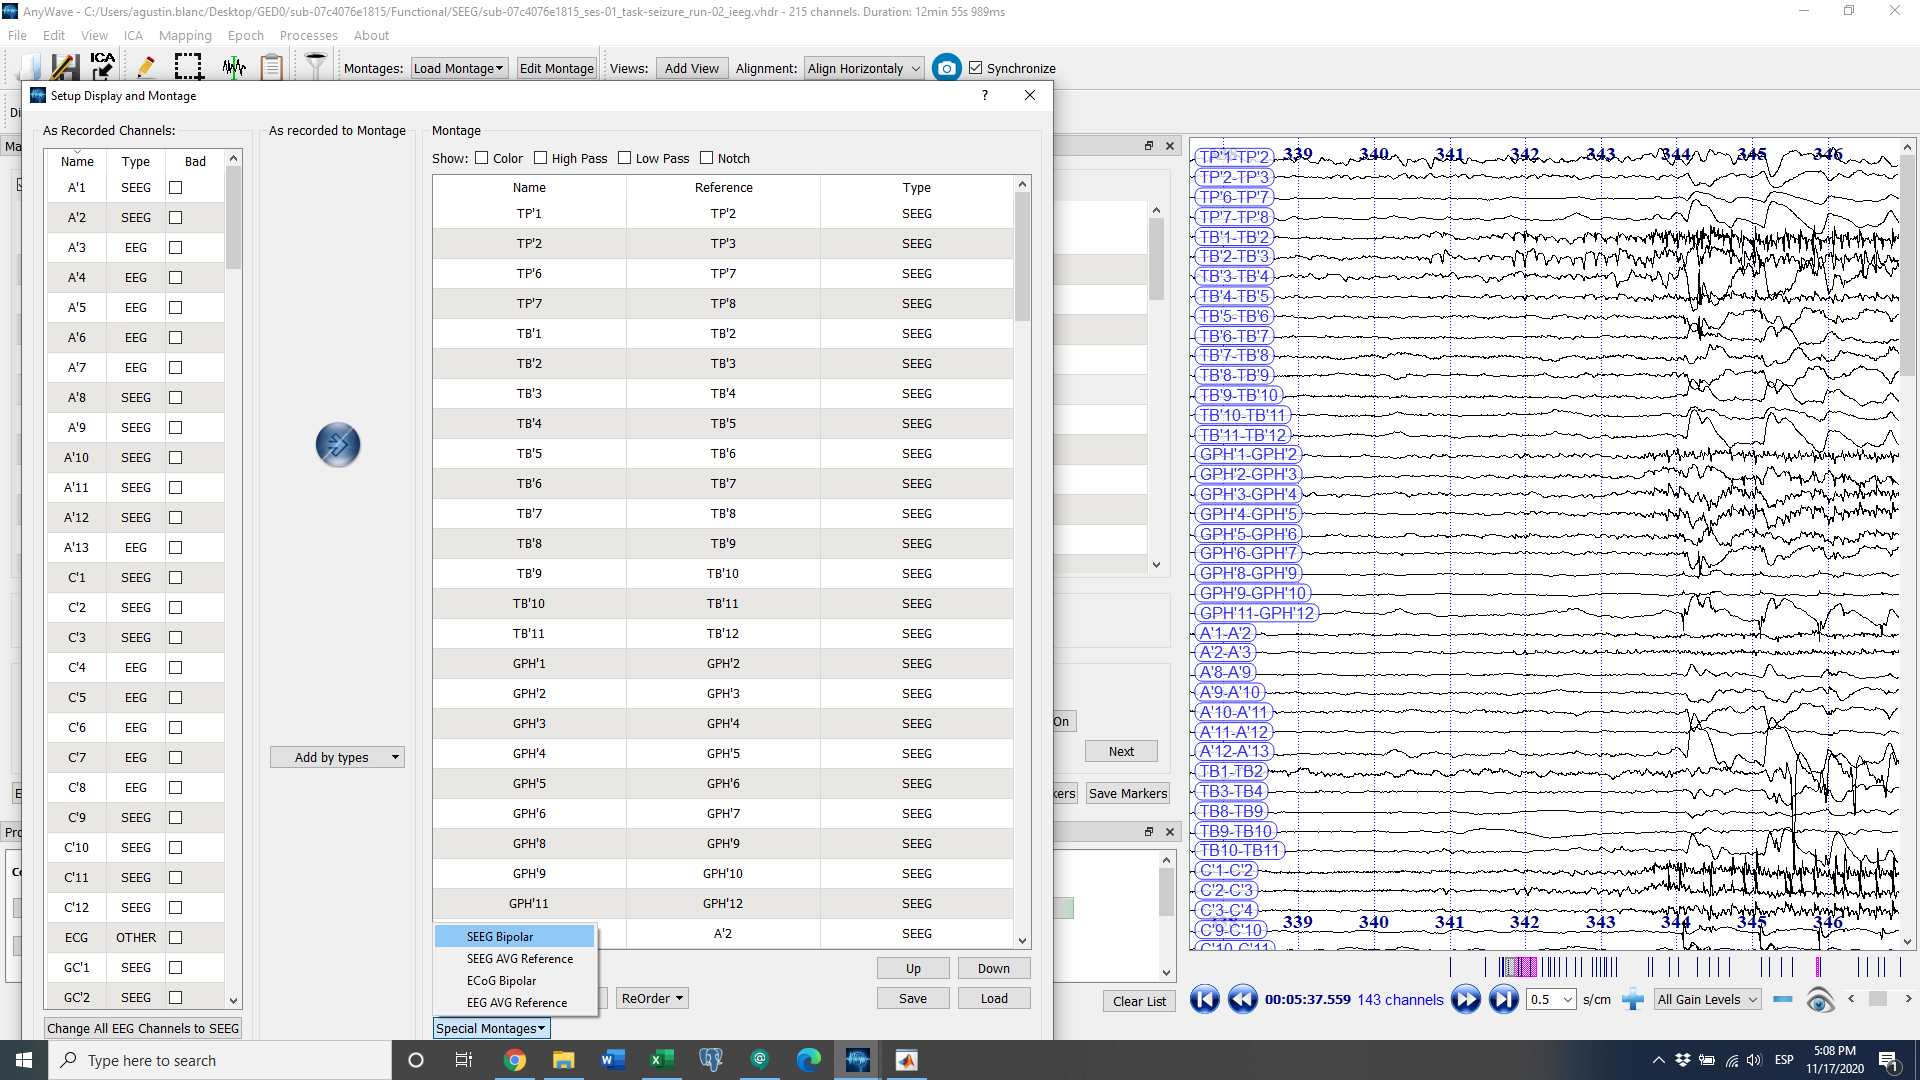
\includegraphics[width=12cm,angle=0]{figures/montage.png} \label{fig:1}
    \caption{Montage display} 
\end{figure}
For the subjects presented in this report, the montages were exported from GARDEL and correspond to the gray matter contacts.

\underline{2. Preprocessing:}

For the preprocessing, we select the ‘Filter’ icon, and a window will pop up. We can define the type of filter, the filtering band and the type of contacts. 

\begin{figure}[H] \hspace{-0cm} \centering \hspace{0cm} 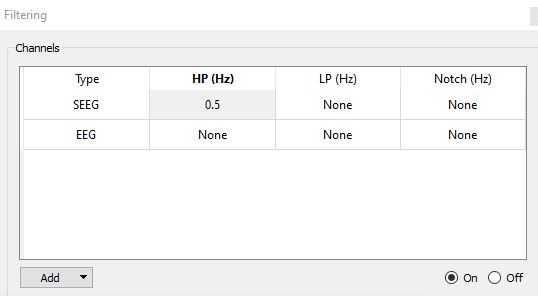
\includegraphics[width=8cm,angle=0]{figures/filter.png} \label{fig:2}
    \caption{Filtering display} 
\end{figure}

For this analysis we used an SEEG HP filter at 0.5 Hz.

\underline{3. Epileptogenicity Index (EI) and Connectivity Epileptogenicity Index (cEI) computing:} 

In order to compute the EI or the cEI, the plugins need to be downloaded and saved in the corresponding folder (Anywave/Plugins/MATLAB). 
The first step is to define the time frame in which the EI/cEI will be computed. For this, we click on the pencil icon for creating a marker, and we select ‘Selection’ for the marker properties and we define ‘EI’ for the label.

\begin{figure}[H] \hspace{-0cm} \centering \hspace{0cm} 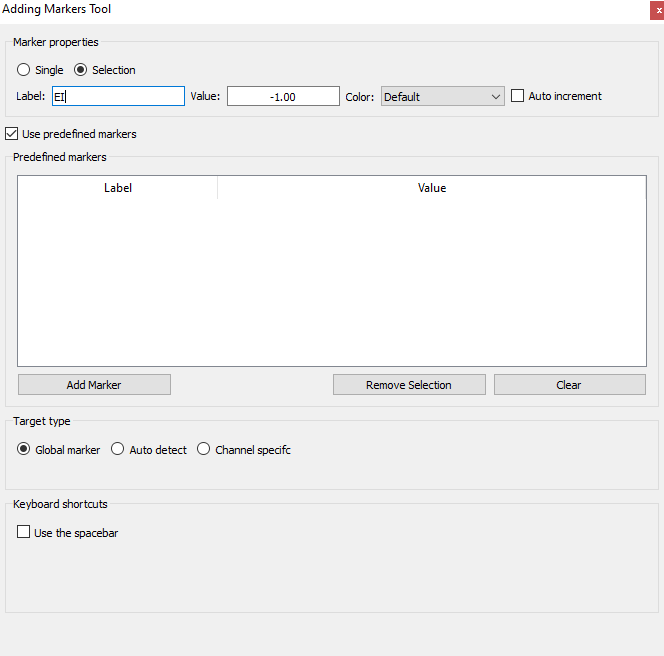
\includegraphics[width=8cm,angle=0]{figures/marker_tool.png} \label{fig:3}
    \caption{Marker display} 
\end{figure}

Then, we can just click on the display of the signals to set the starting and ending point, and a selection in pink will appear to show the created marker. In order to check that it has been created, we can go to View → Markers in the menu and the ‘EI’ selection should be visible. In that panel, we can also edit the length of the marker.

\begin{figure}[H] \hspace{-0cm} \centering \hspace{0cm} 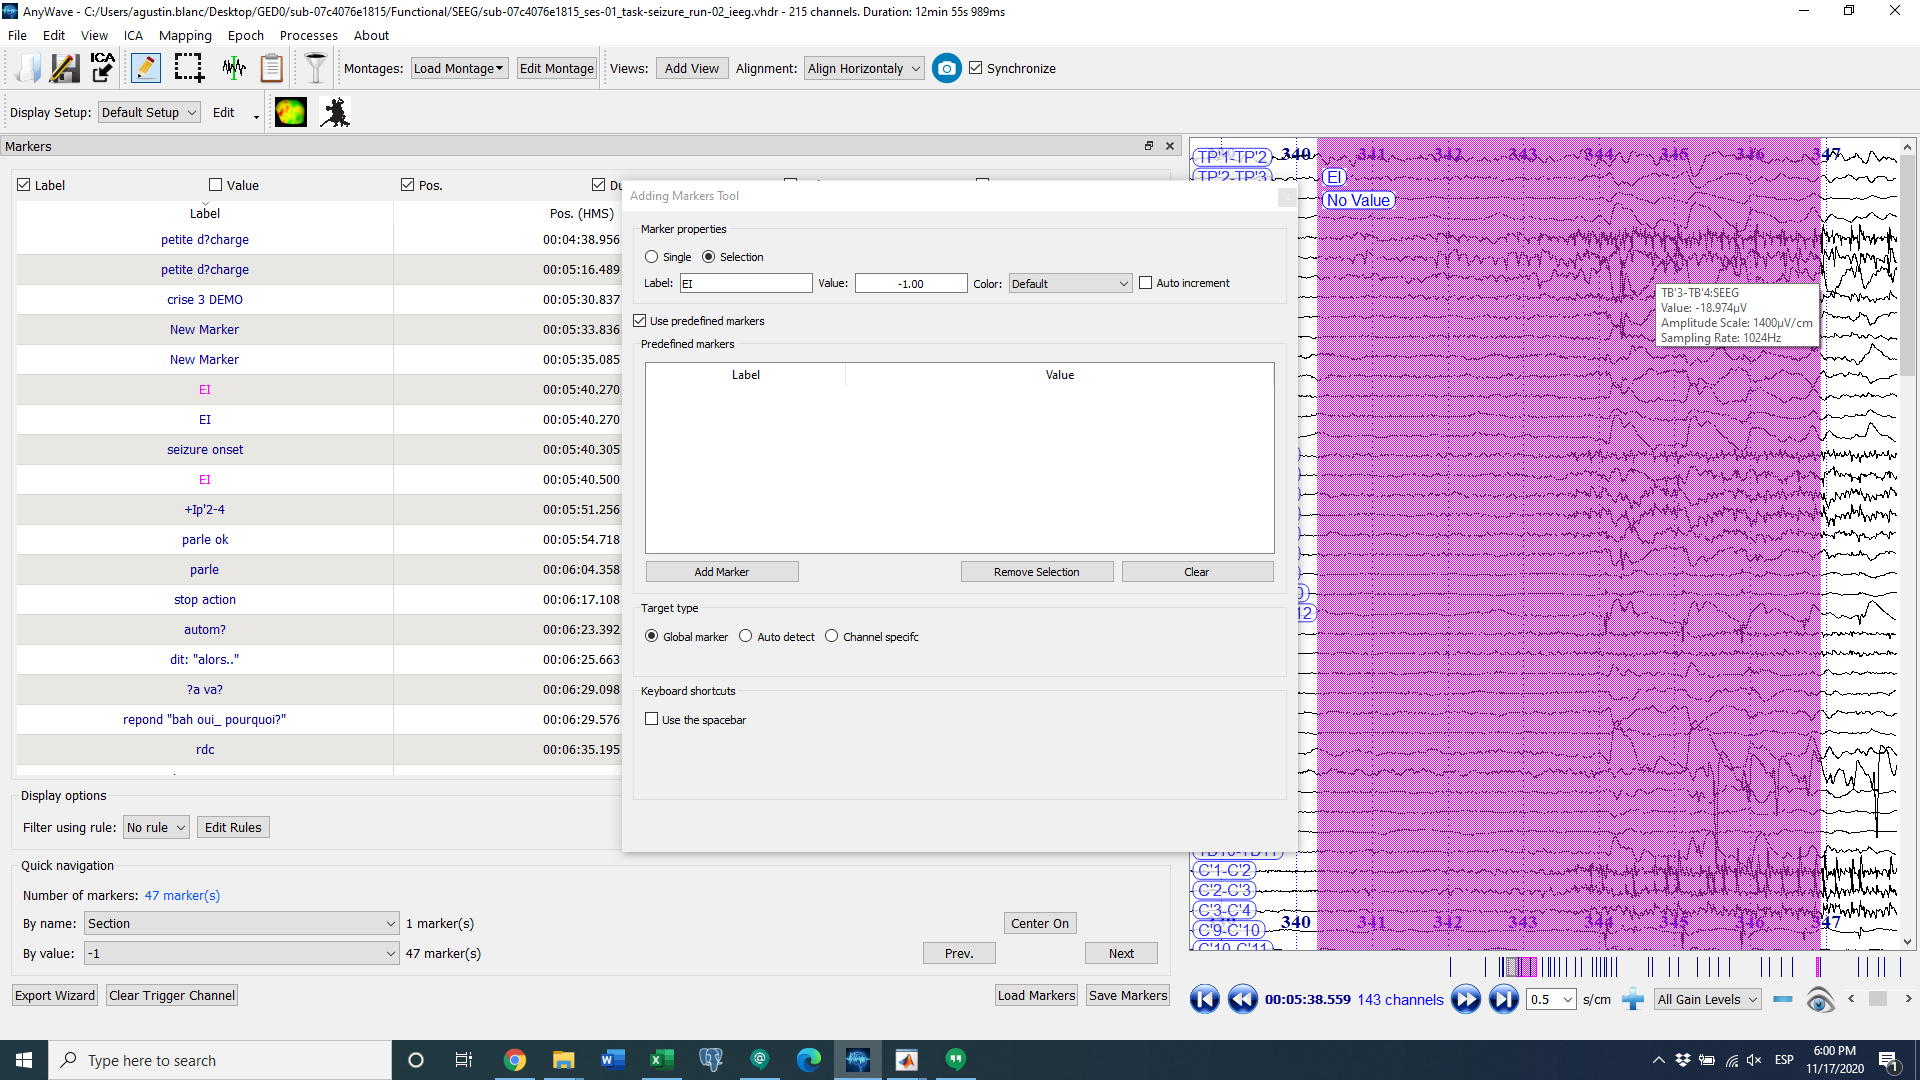
\includegraphics[width=12cm,angle=0]{figures/marker_selection.png} \label{fig:4}
    \caption{EI Marker selection} 
\end{figure}

Typically, we will set the starting point a few seconds before the seizure onset and the duration to 30s.

Once the marker is defined, we can continue to compute the EI/cEI. 

\begin{figure}[H] \hspace{-0cm} \centering \hspace{0cm} 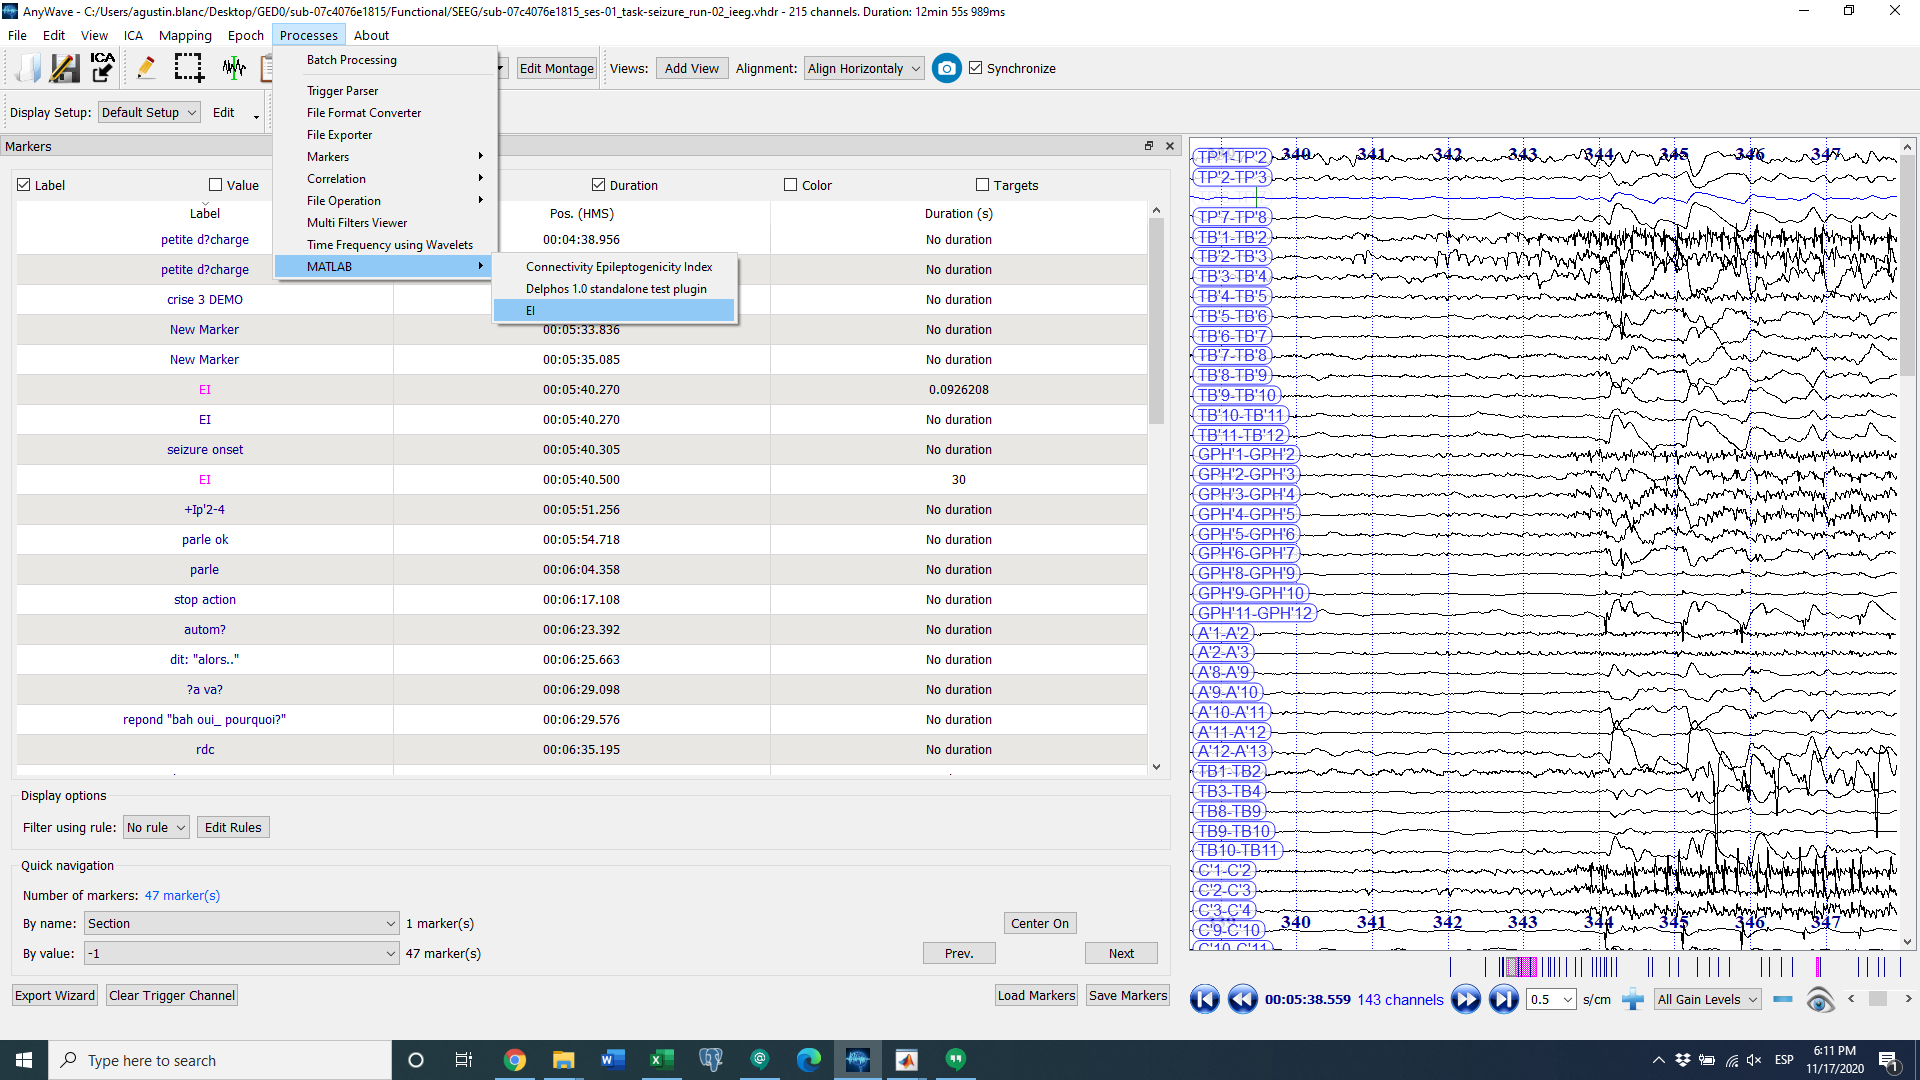
\includegraphics[width=12cm,angle=0]{figures/EI_process.png} \label{fig:5}
    \caption{Computing EI} 
\end{figure}

Once we do this, a new window will appear for the EI/cEI calculations. We can define the ranges for the High Freq. and Low Freq. bands, the detection parameters (bias, decay and threshold) and in the case of the cEI, the algorithm (r2 or h2), the time window, step and max\_lag.

\begin{figure}[H] \hspace{-0cm} \centering \hspace{0cm} 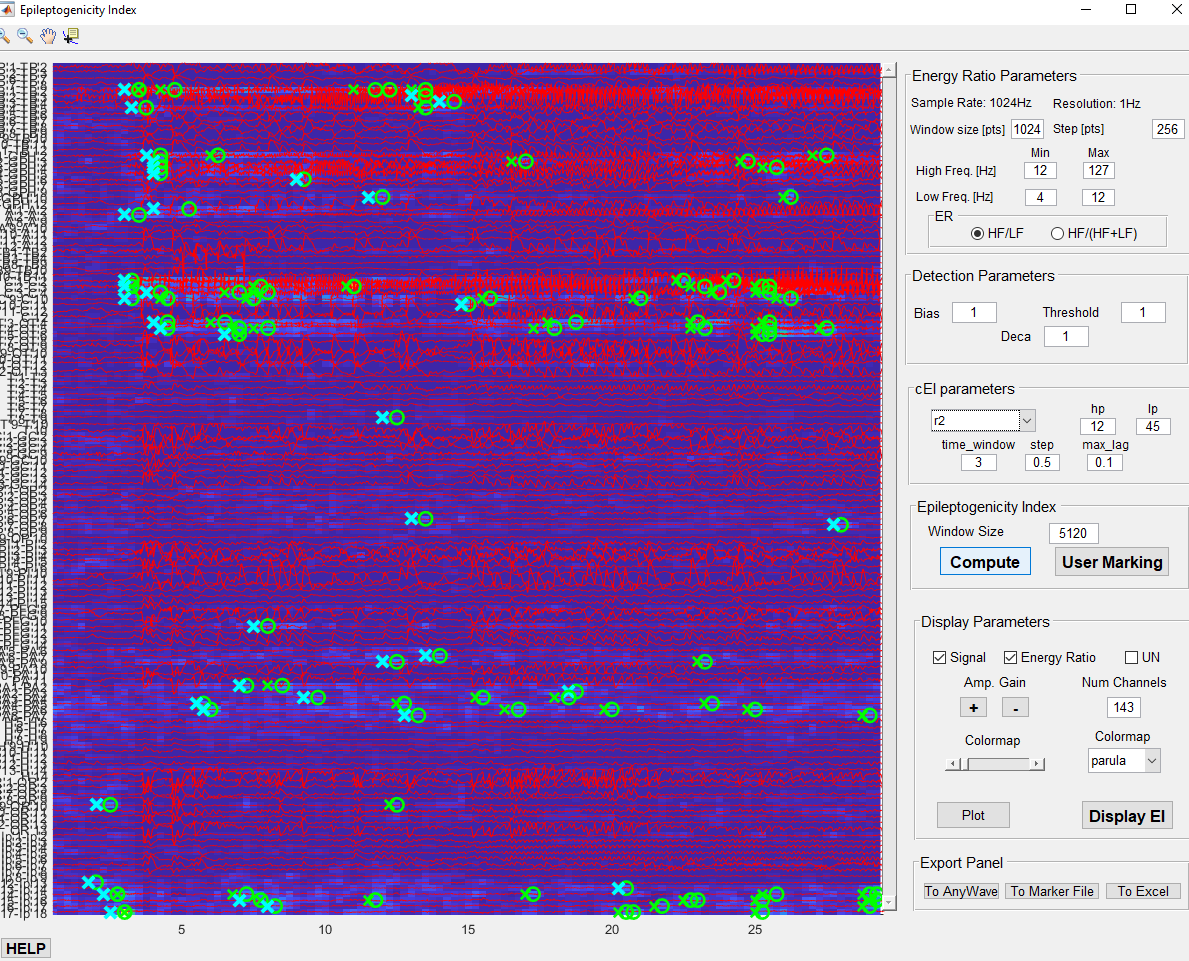
\includegraphics[width=10cm,angle=0]{figures/EI.png} \label{fig:6}
    \caption{EI output display} 
\end{figure}

Then, we click on ‘Compute’ and the plot with all the signals and the detections will appear. If we click on ‘Display EI’, the bar plot with the EI, summed ER and cEI (in the case we have computed it), will be displayed.
From the visual inspection of the signals and the EI detections, we can manually mark the false detections (those signals with physiological high frequencies) to exclude them from the EI calculation.


 \section{Extracting features from ictal SEEG data}
 
 
 \section{Extracting features from interictal SEEG data}

 
%%%%%%%%%%%%%%%%%%%%%%%%%%%%%%%%%%%%%%%%%%%%%%%%
 \section{Features of nodes}
 
 
 
%%%%%%%%%%%%%%%%%%%%%%%%%%%%%%%%%%%%%%%%%%%%%%%
 \section{Features of edges}

%%%%%%%%%%%%%%%%%%%%%%%%%%%%%%%%%%%%%%%%%%%%%%%
\section{Patients description}
\subsection{Patient 8bb}\hfill

\underline{Contacts visualization:} 
  
\begin{figure}[H] \hspace{-0cm} \centering \hspace{0cm} 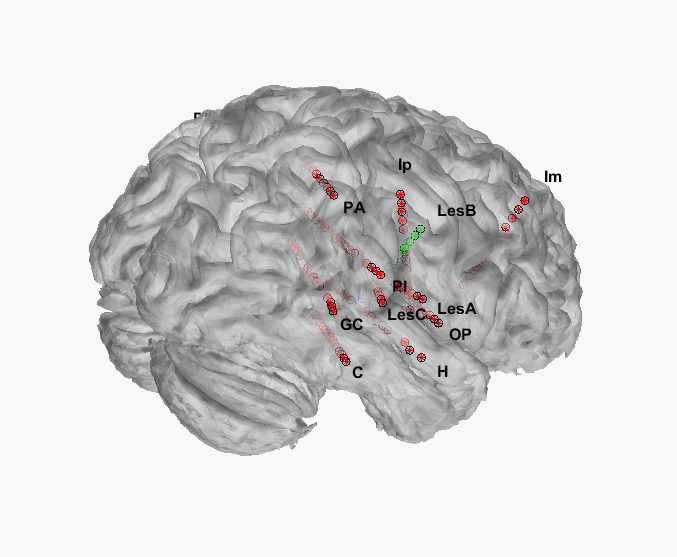
\includegraphics[width=10cm,angle=0]{figures/all_electrodes.png} \label{fig:7}
        \caption{SEEG electrodes visualization} 
      \end{figure}
      
     \begin{figure}[H]
        \centering
        \begin{subfigure}[H]{.4\textwidth}
          \centering
          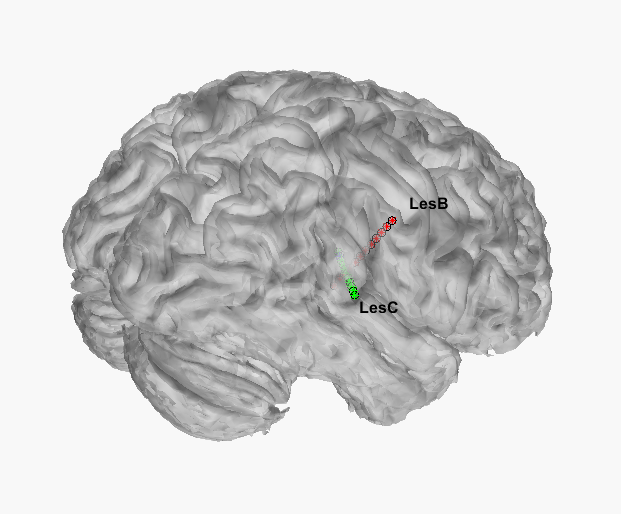
\includegraphics[width=\linewidth]{figures/les_contacts.png}
          \label{fig:sub-first}
        \end{subfigure}
        \begin{subfigure}[H]{.42\textwidth}
          \centering
          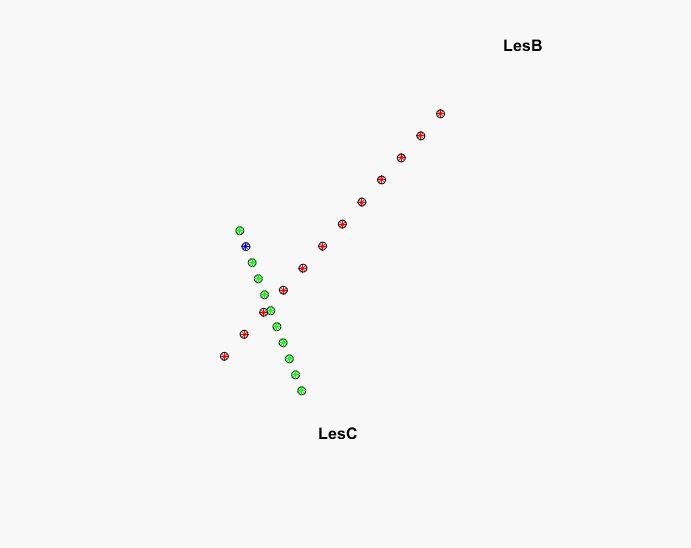
\includegraphics[width=\linewidth]{figures/lesc2.png}  
          \label{fig:sub-second}
        \end{subfigure}
        \caption{Main contacts visualization (LesB2, LesC2)}
        \label{fig:fig8}
      \end{figure}
      
\begin{figure}[H]
        \centering
        \begin{subfigure}[H]{.4\textwidth}
          \centering
          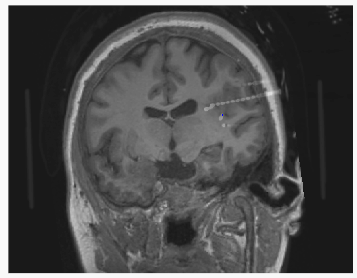
\includegraphics[width=\linewidth]{figures/lesb2.png}
          \caption{LesB2 contact}
           \label{fig:lesb2}
        \end{subfigure}
        \begin{subfigure}[H]{.4\textwidth}
          \centering
          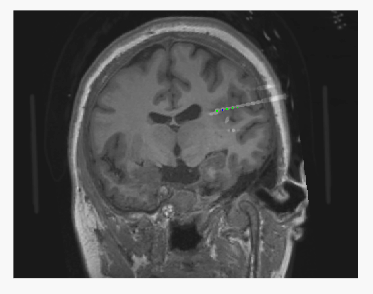
\includegraphics[width=\linewidth]{figures/lesc2_image.png}  
          \caption{LesC2 contact}
          \label{fig:lesc2}
        \end{subfigure}
        \caption{LesB2, LesC2 coronal view}
         \label{fig:fig9}
        \end{figure}


\underline{Seizure 1:}
 
 \begin{figure}[H]
          \centering
          \begin{subfigure}[H]{0.45\textwidth}
            \centering
              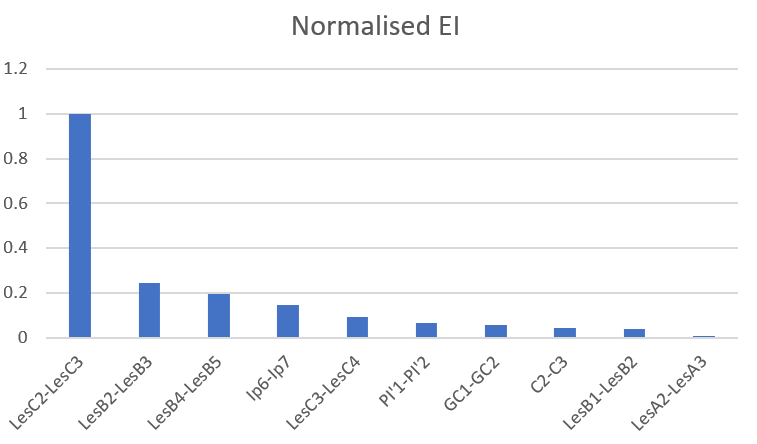
\includegraphics[width=\textwidth]{figures/EI_ord_S1.PNG}
              \label{fig:EI_ordS1}
             \end{subfigure}
             \begin{subfigure}[H]{0.45\textwidth}
              \centering
              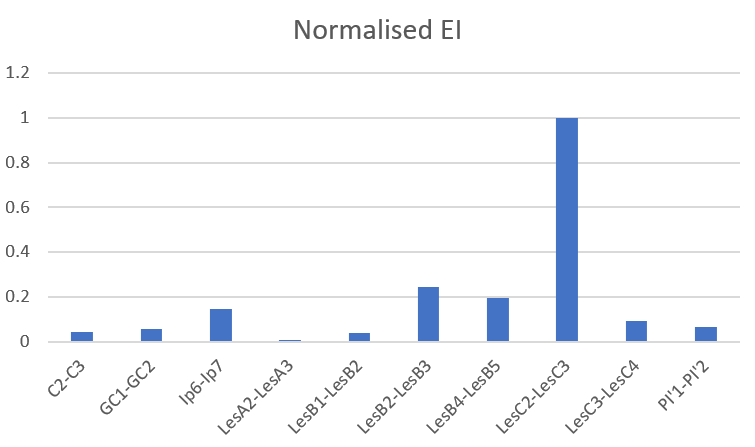
\includegraphics[width=\textwidth]{figures/EI_ch_S1.PNG}
              \label{fig:EI_chS1}
          \end{subfigure}
          \caption{EI Seizure 1}
          \label{fig:10}
        \end{figure}
      
\underline{Seizure 2:}
        
 \begin{figure}[H]
          \centering
          \begin{subfigure}[H]{0.45\textwidth}
            \centering
              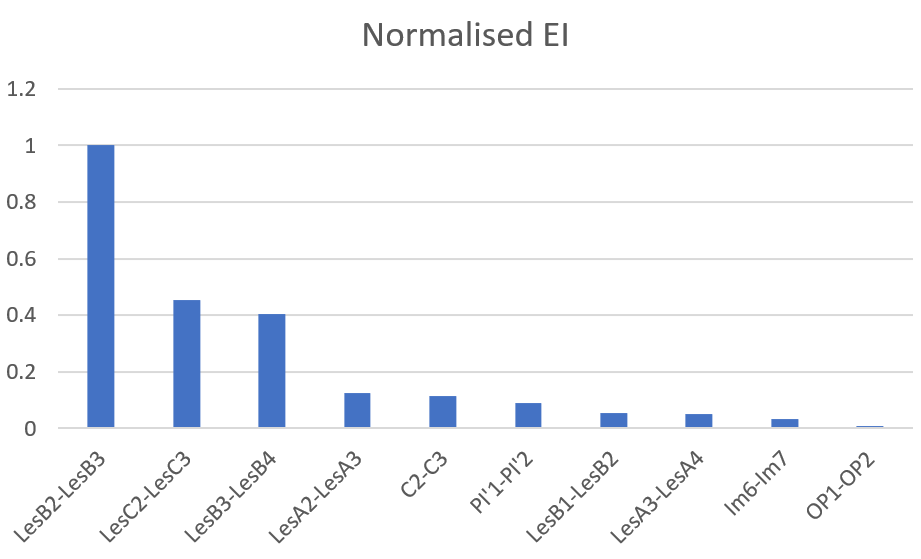
\includegraphics[width=\textwidth]{figures/EI_ord_S2.PNG}
              \label{fig:EI_ordS2}
             \end{subfigure}
             \begin{subfigure}[H]{0.45\textwidth}
              \centering
              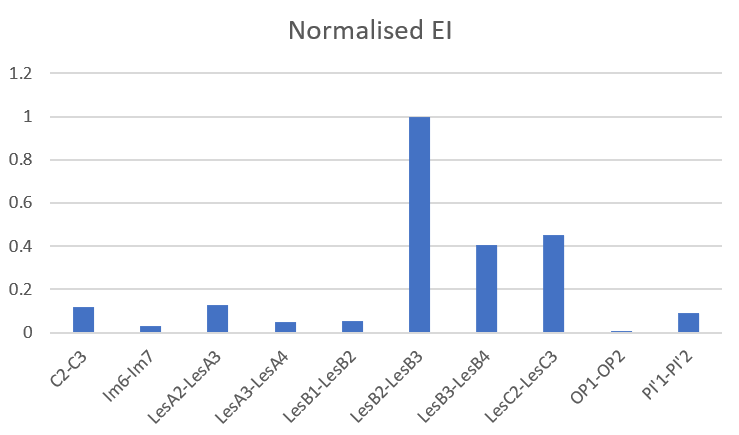
\includegraphics[width=\textwidth]{figures/EI_ch_S2.PNG}
              \label{fig:EI_chS2}
          \end{subfigure}
          \caption{EI Seizure 2}
          \label{fig:11}
        \end{figure}
        
\underline{Seizure 3:}
        
 \begin{figure}[H]
          \centering
          \begin{subfigure}[H]{0.45\textwidth}
            \centering
              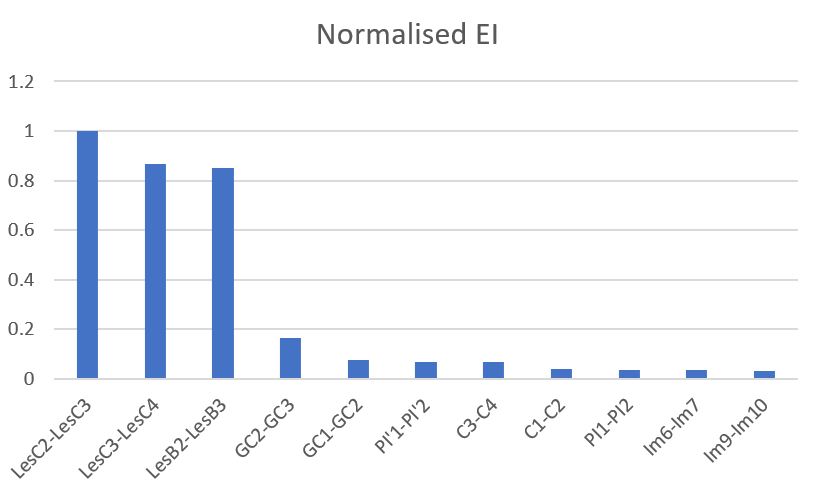
\includegraphics[width=\textwidth]{figures/EI_ord_S3.PNG}
              \label{fig:EI_ordS3}
             \end{subfigure}
             \begin{subfigure}[H]{0.45\textwidth}
              \centering
              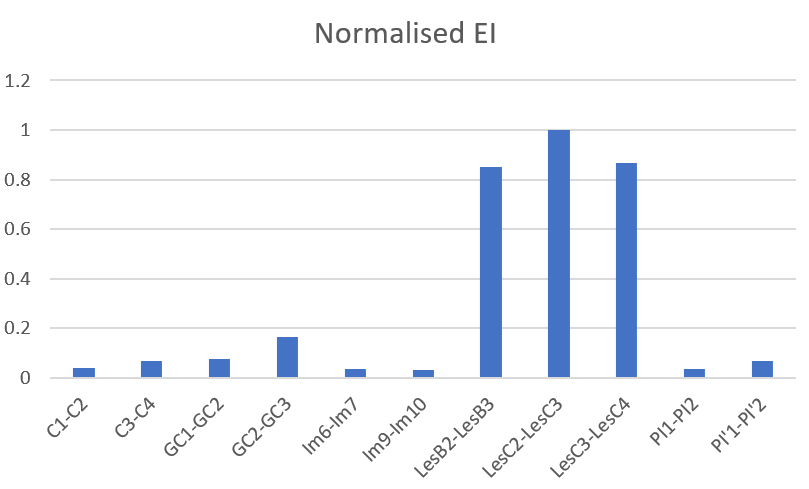
\includegraphics[width=\textwidth]{figures/EI_ch_S3.PNG}
              \label{fig:EI_chS3}
          \end{subfigure}
          \caption{EI Seizure 3}
          \label{fig:12}
        \end{figure}
        
\underline{Average all Seizures:}
        
 \begin{figure}[H] \hspace{-0cm} \centering \hspace{0cm}
    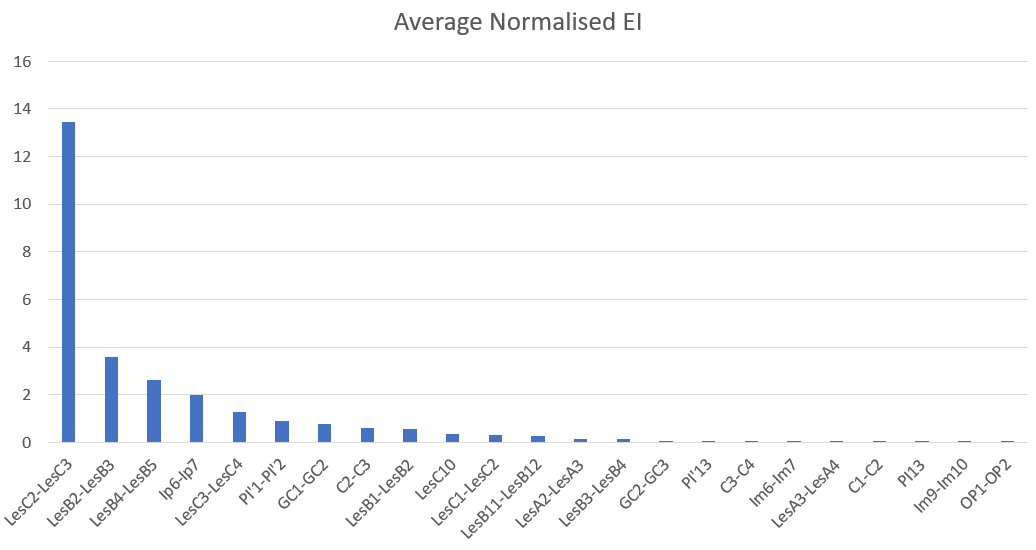
\includegraphics[width=10cm,angle=0]{figures/normalised_EI_allSeiz.PNG} \label{fig:13}
        \caption{Average EI 3 seizures} 
       \end{figure}  
       
We conclude from these plots that C3 and B3 are the most epileptogenic contacts, they belong to L1. But, should we consider them as different nodes? If we look at the 3D plot where we see the localization of the contacts (Fig. \ref{fig:fig8}) they seem to be very close. We can define a distance threshold based on a distance matrix between nodes to define which nodes should be consider from the same region. Moreover, with the help of a parcellation, we can also see if they are localized in the same area. For now, we will assume they are different nodes because there is a time delay between the seizure onset of the two contacts.

Now the question is: How should be define the nodes in L2? A possible rout would be to select the contacts that have non-zero EI. But the contacts that belong to L2 doesn't necessarily have the fast/slow frequency onset profile. Still, the seizure propagates to those nodes. So, it seems like EI may not be the best approach to define L2. 

Moreover, after visual inspection of the time series that have non-zero EI, we hardly see seizure propagation. On the other hand, there are contacts where you can clearly see the propagation (lp5-lp6, for example) and they have an EI of 0. Therefore, there is the need to develop a classifier (pySENT) that will allow us to identify the nodes where the seizure propagates based on (a priori): onset of the seizure (it has to be right after the most epileptogenic contact enters into ictal phase), frequency and amplitude.

\subsection{Patient 07c}


%%%%%%%%%%%%%%%%%%%%%%%%%%%%%%%%%%%%%%%%%%%%%%%%
\section{The pySENT (SEEG NeTork) object}
  
  
\end{document}  
